\documentclass{labo}
\usepackage[utf8x]{inputenc}

\usepackage[english]{babel}
\usepackage[T1]{fontenc}

\usepackage{graphicx}
\usepackage{amssymb}
\usepackage{amsmath}
\usepackage{siunitx}
\usepackage{wasysym} %smiley
\usepackage{textcomp}
% \usepackage{minted}
\usepackage[long]{datetime}
\usepackage{gensymb} % \ohm, celsius
\usepackage{framed}
\usepackage{pdfpages}
\usepackage{paralist}

\usepackage{mathastext} % math as standfard text : units are respecting typography conventions.
\usepackage{fancyhdr} %en-tête
\usepackage{qrcode}
\usepackage{pgfplots} %for latex grid
\usepackage{fontawesome}
\usepackage{charter}

\usepackage{minted}

%%%%%%%%%%%%
% Tables
%%%%%%%%%%%%
\usepackage{dcolumn}
\newcolumntype{.}{D{.}{.}{2}}
\usepackage{booktabs}
\renewcommand{\arraystretch}{1.1} % Opens up the table a tad
\usepackage{multicol}
\usepackage{multirow}

\langexam{frenchb}

\correction{false}
%\correction{true}

\author{}


%% fancy header & foot
\pagestyle{fancy}
\lhead{[4EISA] Image Processing\\ LAB 2 \ifthenelse{\boolean{corrige}}{~-- correction}{}}
\rhead{v1.0.0\\ page \thepage}
\cfoot{}
%%

\pdfinfo{
/Author ()
/Title (4EISA Image Processing, lab 2)
/ModDate (D:\pdfdate)
}

\hypersetup{
pdftitle={LAB 2 [4EISA] Image Processing},
pdfauthor={},
pdfsubject={}
}

\newcommand{\numpy}{\texttt{NumPy} }
\newcommand{\opencv}{\texttt{OpenCV} }

\setminted[python]{
frame=lines,
framesep=2mm,
% baselinestretch=1.2,
fontsize=\small,
linenos,
breaklines
}

\begin{document}

\tptitle{}{Image Processing -- Session 2\\Image transformation and shape detection}

In this session, you will go further in the image processing, still using \opencv and the PiCamera.

\section*{Colourspaces and Real-time tracking}
Before all let’s define the concept of \textbf{colourspace}. A colourspace is a mathematical model used to
represent colours. Usually, colourspaces are used to represent the colours in a numerical form and to
perform mathematical and logical operations with them. The most common one are BGR (\opencv's
default colourspace), RGB, HSV, and greyscale. BGR stands for blue, green, and red. HSV represents
colours in Hue, Saturation, and Value format.\\

To convert an image from one to another colourspace, OpenCV has a function:

\texttt{cv2.cvtColor(img, conv\_flag)} that allows us to change the colourspace of an image \texttt{img}, while the source and target colourspaces are indicated on the \texttt{conv\_flag}\footnote{e.g. \texttt{cv2.COLOR\_BGR2RGB}} parameter. Let’s ask our parrots friends for some help again for the demonstration. Remember that her colours were all wrong the first time we used her in the first lab.
Now try on with this lines:

\begin{minted}{python}
import cv2
import matplotlib.pyplot as plt
img = cv2.imread('parrots.bmp', 1)
img = cv2.cvtColor(img, cv2.COLOR_BGR2RGB)
plt.imshow(img)
plt.title ('COLOR IMAGE')
plt.xticks([])
plt.yticks([])
plt.show()
\end{minted}

Another way to get the same result would be to split the colours into 3 channels, switch the order and merge them back as follow:

\begin{minted}{python}
import cv2
import matplotlib.pyplot as plt
img = cv2.imread('parrots.bmp',1)
b,g,r = cv2.split(img)
img = cv2.merge((r,g,b))
plt.imshow(img)
plt.title ('COLOR IMAGE')
plt.xticks([])
plt.yticks([])
plt.show()
\end{minted}

To access more conversion flags, you may use the following code or simply search in the \opencv library:

\begin{minted}{python}
import cv2
j=0
for filename in dir(cv2):
	if filename.startswith('COLOR_'):
		print(filename)
		j=j+1
print(f"There are {j} Colorspace Conversion flags in OpenCV")
\end{minted}

Now you know how to convert your images into the desired colourspace, let’s see how to
convert and use efficiently those channels to realize a real-time tracking.\\

In HSV format, it's much easier to recognize the colour range. If we need to track a specific
colour object, we will have to define a colour range in HSV, then convert the captured image in the HSV
format, and then check whether the part of that image falls within the HSV colour range of our
interest. We can use the \texttt{cv2.inRange()} function to achieve this. This function takes an image, the upper and lower bounds of the colours, and then checks the range criteria for each pixel. If the pixel
value falls in the given colour range, the corresponding pixel in the output image is 0; otherwise it is
255, thus creating a binary mask.\\

We can use \texttt{bitwise\_and()} to extract the colour range we're interested in using this binary mask thereafter. Take a look at the following code to understand this concept:

\begin{minted}{python}
import numpy as np
import cv2
cam = cv2.VideoCapture(0)
while(True):
	ret, frame = cam.read()
	hsv = cv2.cvtColor(frame, cv2.COLOR_BGR2HSV)
	image_mask = cv2.inRange(hsv, np.array([40,50,50]), np.array([80,255,255]))
	output=cv2.bitwise_and(frame, frame, mask=image_mask)
	cv2.imshow('Original', frame)
	cv2.imshow('Output', output)
	If cv2.waitKey(1) == 27:
		break
cv2.destroyAllWindows()
cam.release()
\end{minted}

We're tracking the {\color{green}green} coloured objects of the camera’s picture in this program.\\

The mask image is not included in the preceding image. You can see it yourself by adding
\texttt{cv2.imshow('Image Mask',image\_mask)} to the code. It would be a binary (pure black and white) image.\\

We can also track multiple colours by tweaking this code a bit. We need to modify the
preceding code by creating a mask for another colour range. Then, we can use \texttt{cv2.add()} to get the combined mask for two distinct colour ranges, as follows:

\begin{minted}{python}
blue = cv2.inRange(hsv, np.array([100,50,50]), np.array([140,255,255]))
green = cv2.inRange(hsv, np.array([40,50,50]), np.array([80,255,255]))
image_mask = cv2.add(blue, green)
output = cv2.bitwise_and(frame, frame, mask=image_mask)
\end{minted}

\begin{leftbar}
Now, try to adapt the code and find out the {\color{blue}blue} and {\color{green}green} M\&Ms from the picture.
\end{leftbar}

\begin{center}
	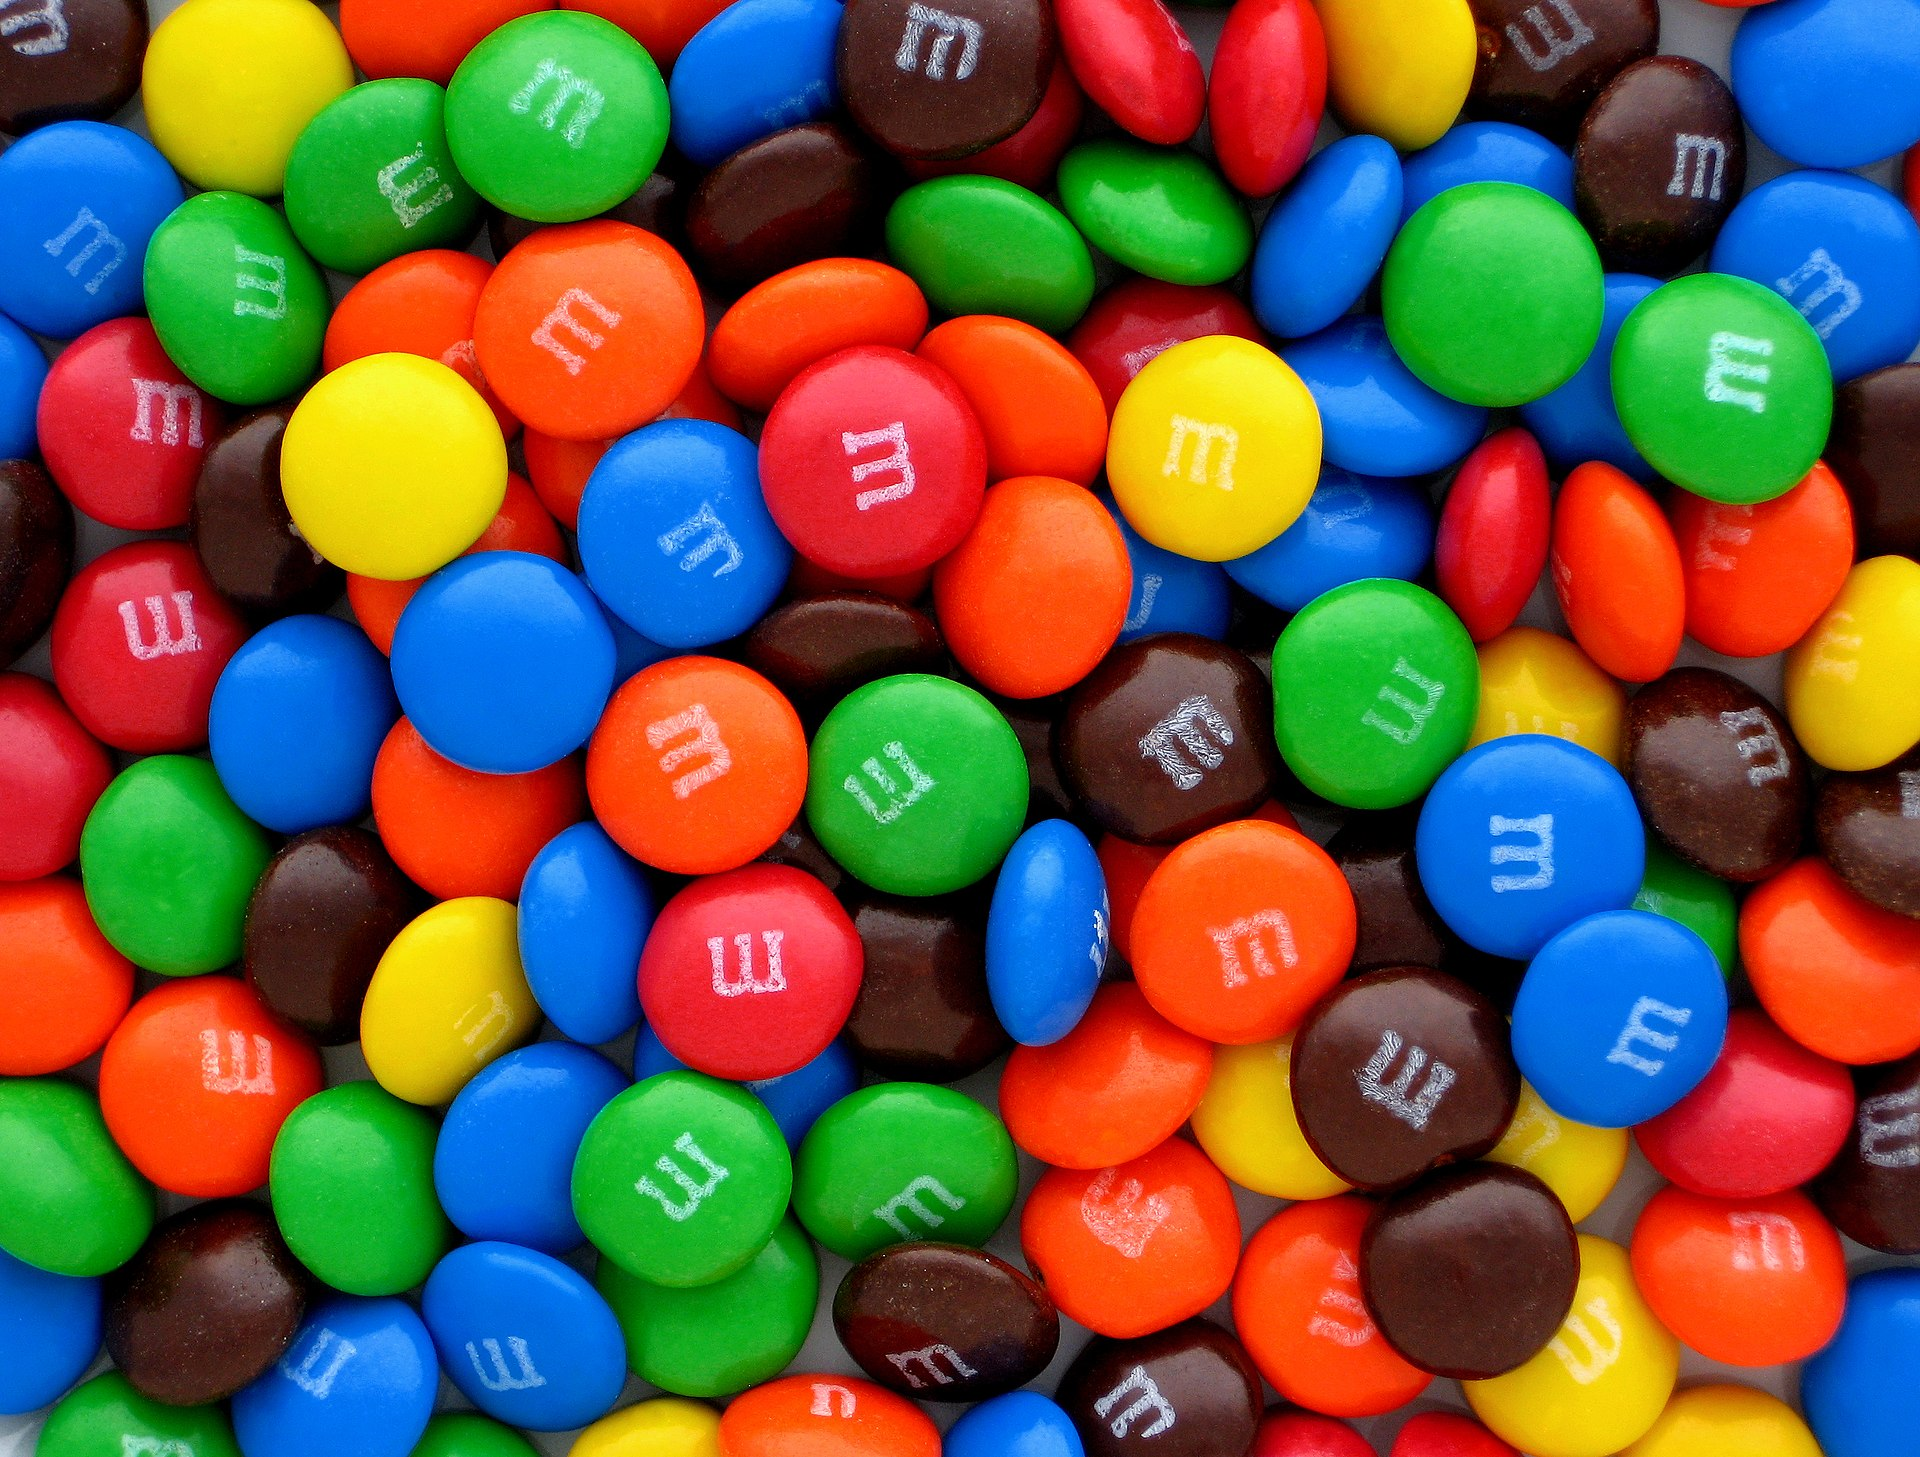
\includegraphics[width=.5\textwidth]{Plain-M&Ms-Pile.jpg}
\end{center}

\section*{Image transformation}
Various transformations can be applied on an image. In this section we will discuss some fundamental ones.

\textbf{Scaling} a picture is the resizing of the image, which can be accomplished by the \texttt{cv2.resize()} function. It takes image, scaling factor, and interpolation method as inputs.
The interpolation method parameter can have any one of the following values:
\begin{description}
	\item[\texttt{INTER\_LINEAR}] This deals with bilinear interpolation (default value)
	\item[\texttt{INTER\_NEAREST}] This deals with the nearest-neighbor interpolation
	\item[\texttt{INTER\_AREA}] This is associated with resampling using pixel area relation (preferred for shrinking)
	\item[\texttt{INTER\_CUBIC}] This deals with bicubic interpolation over 4 x 4 pixel neighborhood (preferred for zooming)
	\item[\texttt{INTER\_LANCZOS4}] This deals with Lanczos interpolation over 8 x 8 pixel neighbourhood
\end{description}

The following example shows the usage for upscaling and downscaling:

\begin{minted}{python}
import cv2
img = cv2.imread('img.png',1)
UpScale = cv2.resize(img,None,fx=1.5,fy=1.5, interpolation=cv2.INTER_CUBIC) 
DownScale = cv2.resize(img,None,fx=0.5,fy=0.5, interpolation=cv2.INTER_AREA) 
cv2.imshow('upscale',UpScale) 
cv2.waitKey(0) cv2.imshow('downscale',DownScale)
cv2.waitKey(0) 
cv2.destroyAllWindows()
\end{minted}

In the preceding code, we upscale the image in the x and y axes with a factor of 1.5 and downscale in x and y axes with a factor of 0.5. Run the code and see the output for yourself.\\

\textbf{Translation, rotation, and affine transformation} can be performed with the function \texttt{cv2.warpAffine()}. It takes an input image, transformation matrix, and size of the output image as inputs, and returns the transformed image.\\

\textbf{Translation} means shifting the location of the image. The shifting factor in (x,y) can be denoted with the transformation matrix, as follows:
\[ T = 
\begin{bmatrix}
1 & 0 & x\\
0 & 1 & y
\end{bmatrix}
\]

The following code shifts the location of the image with (-50,50):

\begin{minted}{python}
import numpy as np 
import cv2 
import matplotlib.pyplot as plt 
img = cv2.imread('img.png',1) 
input = cv2.cvtColor(img,cv2.COLOR_BGR2RGB) 
rows,cols,channel = img.shape 
T = np.float32([[1,0,-50],[0,1,50]]) 
output = cv2.warpAffine(input,T,(cols,rows)) 
plt.imshow(output)
plt.title('Shifted Image') 
plt.show()
\end{minted}

Some parts of the image will be cropped as the size of the output is the same as the input. Similarly, we can use \texttt{cv2.warpAffine()} to apply scaled rotation to an image. For this, we need to define a rotation matrix with the use of \texttt{cv2.getRotationMatrix2D()}, which accepts the centre of the rotation, the angle of anti-clockwise rotation (in degrees), and the scale as parameters, and provides a rotation matrix, which can be specified as the parameter to \texttt{cv2.warpAffine()}. \\

The following example rotates the image by 45 degrees with the centre of the image as the centre of rotation, and scales it down to 50\% of the original image:

\begin{minted}{python}
import cv2 
import matplotlib.pyplot as plt 
img = cv2.imread('img.png',1) 
input = cv2.cvtColor(img,cv2.COLOR_BGR2RGB) 
rows,cols,channel = img.shape 
R = cv2.getRotationMatrix2D((cols/2,rows/2),45,0.5) 
output = cv2.warpAffine(input,R,(cols,rows)) 
plt.imshow(output)
plt.title('Rotated and Downscaled Image') 
plt.show()
\end{minted}
We can create some animation or visual effects by changing the rotation angle at regular intervals and then displaying it in a continuous loop till the \texttt{Esc} key is pressed. Following is the code for this (check the output yourself):

\begin{minted}{python}
import cv2 
from time import sleep 
image = cv2.imread('parrots.bmp',1) 
rows,cols,channels = image.shape 
angle = 0 
while(1): 
	if angle == 360: 
		angle=0 
	M = cv2.getRotationMatrix2D((cols/2,rows/2),angle,1) 
	rotated = cv2.warpAffine(image,M,(cols,rows)) 
	cv2.imshow('Rotating Image',rotated) 
	angle = angle+1 
	sleep(0.05) 
	if cv2.waitKey(1) == 27: 
		break 
cv2.destroyAllWindows()
\end{minted}

\begin{leftbar}
Try implementing this on the live cam.
\end{leftbar}

Next, we will see how to implement an \textbf{affine transformation} on any image. An affine transformation is a function between affine spaces. After applying the affine transformation on an image, the parallelism between the lines in an image is preserved. This means that the parallel lines in original images remain parallel even after transformation. The affine transformation needs any three non-collinear points (points which are not on the same line) in the original image and the corresponding points in the transformed image. These points are passed as arguments to \texttt{cv2.getAffineTransform()} to get the transformation matrix, and that matrix, in turn, is passed to \texttt{cv2.warpAffine()} as an argument. Take a look at the following example:

\begin{minted}{python}
import cv2 
import numpy as np 
import matplotlib.pyplot as plt 
image = cv2.imread('parrots.bmp',1) 
#changing the colorspace from BGR->RGB 
input = cv2.cvtColor(image, cv2.COLOR_BGR2RGB ) 
rows,cols,channels = input.shape 
points1 = np.float32([[100,100],[300,100],[100,300]]) 
points2 = np.float32([[200,150],[400,150],[100,300]]) 
A = cv2.getAffineTransform(points1,points2) 
output = cv2.warpAffine(input,A,(cols,rows)) 
plt.subplot(121)
plt.imshow(input)
plt.title('Input') 
plt.subplot(122)
plt.imshow(output)
plt.title('Affine Output') 
plt.show()
\end{minted}

As we often say\dots~ ``changing our perspective'' can offer us some opportunities. This modification is also available in image processing. The \textbf{perspective transformation} needs four points in an input image and four corresponding point in the output image\footnote{Three of the points cannot be collinear, in other words, three out of the four point cannot be part of a straight line.}. A real-life example would be a numerical zoom on a picture.\\

To get a better idea of the \textbf{perspective transformation}, let’s write it in a code. We will use \texttt{cv2.getPerspectiveTransform()} to generate the transformation matrix and \texttt{cv2.warpPerspective()} to get the transformed output:

\begin{minted}{python}
import cv2 
import numpy as np 
import matplotlib.pyplot as plt 
image = cv2.imread('parrots.bmp',1) 
#changing the colorspace from BGR->RGB 
input = cv2.cvtColor(image, cv2.COLOR_BGR2RGB) 
rows,cols,channels = input.shape 
points1 = np.float32([[0,0],[400,0],[0,400],[400,400]]) 
points2 = np.float32([[0,0],[300,0],[0,300],[300,300]]) 
P = cv2.getPerspectiveTransform(points1,points2) 
output = cv2.warpPerspective(input,P,(300,300)) 
plt.subplot(121)
plt.imshow(input)
plt.title('Input') 
plt.subplot(122)
plt.imshow(output)
plt.title('Perspective Transform') 
plt.show()
\end{minted}

\begin{leftbar}
Try passing various combination of the parameters to see how the resultant image changes. In the preceding example, parallelism between the lines is preserved because of the combination of the parameters we used. Try different combinations of the parameters to see that the parallelism between the lines is not preserved.
\end{leftbar}

\textbf{Thresholding} is a simple way to segment images\footnote{Best on greyscale images but algorithms are also available for coloured images.}. Usually, the thresholding is the first step to perform in image processing and it converts the greyscale into a binary image of black and white but some algorithms maintain some level of grey. \\

To perform a thresholding, you first need to define the threshold in a greyscale intensity for which all the pixel will be compared with. For example, if the value of the pixel is above the threshold, the pixel becomes white and black otherwise\footnote{The decision of conversion into black or white is arbitrarily defined in the code.}. \\

In \opencv, the \texttt{cv2.threshold()} function is used to threshold images. It takes as inputs: greyscale image, threshold value, maxVal, and threshold method, and returns the thresholded image as output. The maxVal parameter is the value assigned to the pixel if the pixel intensity is greater (or less in some methods) than the threshold. There are five threshold methods available in \opencv; in the beginning, the simplest form of thresholding we saw is \texttt{cv2.THRESH\_BINARY}. Let's see the mathematical representation of all the threshold methods.\\

Say (x,y) is the input pixel; then, operations by threshold methods are as follows:
\begin{description}
	\item[\texttt{cv2.THRESH\_BINARY}] If intensity(x,y) > thresh, then set intensity(x,y) = maxVal; else set intensity(x,y) = 0. 
	\item[\texttt{cv2.THRESH\_BINARY\_INV}] If intensity(x,y) > thresh, then set intensity(x,y) = 0; else set intensity(x,y) = maxVal.
	\item[\texttt{cv2.THRESH\_TRUNC}]  If intensity(x,y) > thresh, then set intensity(x,y)=threshold; else leave intensity(x,y) as it is.
	\item[\texttt{cv2.THRESH\_TOZERO}] If intensity(x,y)> thresh; then leave intensity(x,y) as it is; else set intensity(x,y) = 0.
	\item[\texttt{cv2.THRESH\_TOZERO\_INV}] If intensity(x,y) > thresh, then set intensity(x,y) = 0; else leave intensity(x,y) as it is.
\end{description}

Let’s try it in an example by choosing the value of the threshold as 127, so the image is segmented into two sets of pixels depending on the value of their intensity:

\begin{minted}{python}
import cv2 
import matplotlib.pyplot as plt 
img = cv2.imread('parrots.bmp',0) 
th = 127 
max_val = 255 
ret,o1 = cv2.threshold(img,th,max_val,cv2.THRESH_BINARY) 
ret,o2 = cv2.threshold(img,th,max_val,cv2.THRESH_BINARY_INV) 
ret,o3 = cv2.threshold(img,th,max_val,cv2.THRESH_TOZERO) 
ret,o4 = cv2.threshold(img,th,max_val,cv2.THRESH_TOZERO_INV) 
ret,o5 = cv2.threshold(img,th,max_val,cv2.THRESH_TRUNC) 
titles = ['Input Image','BINARY','BINARY_INV','TOZERO','TOZERO_INV','TRUNC']
output = [img, o1, o2, o3, o4, o5] 
for i in range(6): 
	plt.subplot(2,3,i+1)
	plt.imshow(output[i],cmap='gray') 
	plt.title(titles[i]) 
	plt.xticks([])
	plt.yticks([]) 
plt.show()
\end{minted}

Other methods exist such as the Otsu’s method\footnote{Discussed in the reference book}. For more information, you may be interested to look into the \href{https://docs.opencv.org/4.x/d7/d4d/tutorial_py_thresholding.html}{OpenCV library}. A nice function to use is the \texttt{cv2.adaptiveThreshold()}, which is used for adaptive thresholding of images based on uneven lighting conditions.


\section*{Edge detection}
High-pass filters (HPF) will let high-frequency information like edges to enhance, while restricting low-frequency information. These filters are also called derivative masks and are widely used in edge detection and extraction algorithms. We will study three derivative functions available in OpenCV and see how these are useful in the extracting of edges. \opencv provides the \texttt{Sobel()}, \texttt{Laplacian()}, and \texttt{Scharr()} functions for high-pass filtering.\\

Before speaking of HPF, we need to define the Kernel in image processing:
\[K = \frac{\text{all ones matrix of size }[\text{rows}, \text{columns}]}{\text{rows} \times \text{columns}} \]

For rows = columns = 3, we thus have:
\[K = \frac{
\begin{bmatrix}
1 & 1 & 1\\
1 & 1 & 1\\
1 & 1 & 1
\end{bmatrix}
}{\text{rows} \times \text{columns}} \]

The following are the most common parameters used in the functions mentioned before:

\begin{description}
	\item[\texttt{src}] This is the source image. 
	
	\item[\texttt{ddepth}] This is the depth of the target image. -1 stands for the same depth of target as that of the source. The following combinations of source image depth and target image depth are supported by \texttt{Sobel()}, \texttt{Laplacian()}, and \texttt{Scharr()} derivatives.
	\begin{center}
	\begin{tabular}{ll}\toprule
	Source image depth & Target image depth\\
	\midrule
	CV\_8U & -1/CV\_16S/CV\_32F/CV\_64F \\
	CV\_16U/CV\_16S & -1/CV\_32F/CV\_64F \\
	CV\_32F & -1/CV\_32F/CV\_64F \\
	CV\_64F & -1/CV\_64F \\
	\bottomrule
	\end{tabular}
	\end{center}
	\item[\texttt{dx}] This is the order of the x derivative (not required for Laplacian()).
	\item[\texttt{dy}] This is the order of the y derivative (not required for Laplacian()).
	\item[\texttt{ksize}] This is the kernel size (1,3,5,7 for \texttt{sobel()}, a positive odd number for \texttt{Laplacian()}, and is not required for \texttt{Scharr()}).
	\item[\texttt{scale}] This is the optional scale for computed derivative values.
	\item[\texttt{delta}] This is the optional delta value that is added to the results prior to storing them in the output.
	\item[\texttt{borderType}] This is the pixel extrapolation method for boundary pixels.
\end{description}

Let's see the code in action for \texttt{Sobel()}, \texttt{Laplacian()}, and \texttt{Scharr()}. In the following code, we will compute the Laplacian of the image as well as the first-order x derivative, using the \texttt{Scarr()} and \texttt{Sobel()} functions:

\begin{minted}{python}
import cv2 
import matplotlib.pyplot as plt 
img = cv2.imread('parrots.bmp',0) 
laplacian = cv2.Laplacian(img,ddepth=cv2.CV_32F, ksize=17,scale=1,delta=0,borderType=cv2.BORDER_DEFAULT) 
sobel = cv2.Sobel(img,ddepth=cv2.CV_32F,dx=1,dy=0, ksize=11,scale=1,delta=0,borderType=cv2.BORDER_DEFAULT) 
scharr = cv2.Scharr(img,ddepth=cv2.CV_32F,dx=1,dy=0,scale=1, delta=0,borderType=cv2.BORDER_DEFAULT) 
images=[img,laplacian,sobel,scharr] 
titles=['Original','Laplacian','Sobel','Scharr'] 
for i in range(4): 
	plt.subplot(2,2,i+1) 
	plt.imshow(images[i],cmap = 'gray') 
	plt.title(titles[i])
	plt.xticks([])
	plt.yticks([]) 
plt.show()
\end{minted}

\begin{leftbar}
As an exercise, compute the first-order y derivatives of the image using the Sobel and Scharr functions. Then, use the \texttt{cv2.add()} function to add the Sobel x derivative to the Sobel y derivative. In the same way, add the Scharr x derivative to the Scharr y derivative of the same image and compare the results.
\end{leftbar}

The Canny edge detector detector is a multistage edge detection method developed by John Canny. \opencv implements it using \texttt{cv2.Canny()}. It works in the following stages: 


\begin{enumerate}
	\item A Gaussian kernel is applied to filter out any noise. A 5x5 kernel is used. 

	\item The intensity gradient of the image is calculated. If \texttt{L2gradient} is true, then the L2 norm is used, and if it's false, then the L1 norm is used. 

	\item Non-maximum suppression is applied to the output of step 2 and the candidate edges are identified. 

	\item The final step involves hysteresis. The values of \texttt{threshold1} and \texttt{threshold2} are passed to the function. Anything with a gradient below \texttt{threshold1} is excluded and anything with a gradient that is more than \texttt{threshold2} is included in the edge set. For the points in which the gradient lies between two thresholds, only the pixels that are connected to the pixels that lie above \texttt{threshold2} are accepted as part of the final edge set.
\end{enumerate}

The following parameters are usually passed to \texttt{cv2.Canny()}:
\begin{description}
	\item[\texttt{img}] This is the input image.
	\item[\texttt{threshold1}] This is the lower threshold.
	\item[\texttt{threshold2}] This is the upper threshold.
	\item[\texttt{L2gradient}] This is a Boolean value. If it's True, then the L2 norm is used. Otherwise, the L1 norm is used to calculate the gradient. Usually, the L2 norm is more accurate than the L1 norm, but the former requires more time for computation.
\end{description}

The function will return a set with the detected edges.
The following code will compute and display the edges with the help of the Canny detector:

\begin{minted}{python}
import cv2 
import matplotlib.pyplot as plt 
img = cv2.imread('parrots.bmp',0) 
edges1 = cv2.Canny(img,50,300,L2gradient=False) 
edges2 = cv2.Canny(img,100,150,L2gradient=True) 
images = [img,edges1,edges2] 
titles = ['Original','L1 Gradient','L2 Gradient'] 
for i in range(3): 
	plt.subplot(1,3,i+1) 
	plt.imshow(images[i],cmap = 'gray') 
	plt.title(titles[i])
	plt.xticks([])
	plt.yticks([])
plt.show()
\end{minted}



\section*{Circle detection}
\opencv has \texttt{cv2.HoughCircles()} to detect the circle feature in an image, and it returns the circles in the images in the form of a vector (x, y, radius). It accepts the following parameters as arguments:

\begin{itemize}
	\item An image: This is an 8-bit single-channel greyscale. 

	\item The detection method: This is the method for circle detection. As of now, only one method, \texttt{cv2.HOUGH\_GRADIENT}, has been implemented. 

	\item $dp$: This is the inverse ratio of resolution. This is the formula:
	\[ dp = \frac{\text{image resolution}}{\text{accumulator resolution}} \]

	\item \texttt{minDist}: This is the minimum distance between the centers of the detected circles. 

	\item \texttt{param1} and \texttt{param2}: These are the method-specific parameters. The \texttt{param1} method is the highest threshold of the underlying Canny method, and the \texttt{param2} method is the accumulator threshold for \texttt{HOUGH\_GRADIENT}. 

	\item \texttt{minRadius} and \texttt{maxRadius}: These are the respective parameters for the minimum and maximum radius of the circles for detection.
\end{itemize}

The following program accepts the feed from the webcam and then smooths the image by blurring it, before passing it to \texttt{cv2.HoughCircles()}. The detected circles are drawn using \texttt{cv2.Circle()}, which is something that we have already seen in the previous lab session:

\begin{minted}{python}
import cv2
cam = cv2.VideoCapture(0) 
while (True): 
	ret, frame = cam.read() 
	grey = cv2.cvtColor(frame,cv2.COLOR_BGR2GRAY) 
	blur = cv2.blur(grey,(5,5)) 
	circles = cv2.HoughCircles(blur, method=cv2.HOUGH_GRADIENT,dp=1,minDist=200, param1=50,param2=13,minRadius=30,maxRadius=175) 
	if circles is not None: 
		for i in circles[0,:]:
			i = list(map(int, i))
			cv2.circle(frame,(i[0],i[1]),i[2],(0,255,0),2) 
			cv2.circle(frame,(i[0],i[1]),2,(0,0,255),3) 
			cv2.imshow('Detected',frame) 
	if cv2.waitKey(5) == 27: 
		break 
cv2.destroyAllWindows() 
cam.release()
\end{minted}

\begin{leftbar}
Try it with several balls in the lab and adapt it to the example images.
\end{leftbar}

\opencv also has a \texttt{cv2.HoughLines()} function to find the lines. Let's see how we can detect lines in a live video feed.\\

In the following example, \texttt{cv2.HoughLines()} accepts the following parameters:
\begin{itemize}
	\item An image: This is an 8-bit single-channel greyscale image 
	\item The rho value ($\rho$): This is the distance accuracy of an accumulator 
	\item The theta value ($\theta$): This is the angle accuracy of an accumulator 
	\item The threshold: This is the accumulator threshold parameter
\end{itemize}

This function returns lines in the ($\rho,\theta$) vector that we need to convert to the (x1,y1),(x2,y2) system:

\begin{minted}{python}
import cv2 
import numpy as np 
cam = cv2.VideoCapture(0) 
while (1): 
	ret, img = cam.read() 
	gray = cv2.cvtColor(img,cv2.COLOR_BGR2GRAY) 
	edges = cv2.Canny(gray,50,250,apertureSize=5,L2gradient=True) 
	lines = cv2.HoughLines(edges,1,np.pi/180,200) 
	if lines is not None: 
		for rho,theta in lines[0]: 
			a = np.cos(theta) 
			b = np.sin(theta) 
			x0 = a*rho 
			y0 = b*rho 
			pts1 = ( int(x0 + 1000*(-b)) , int(y0 + 1000*(a)) ) 
			pts2 = ( int(x0 - 1000*(-b)) , int(y0 - 1000*(a)) ) 
			cv2.line(img,pts1,pts2,(0,0,255),2) 
			cv2.imshow('Detected Lines',img) 
	if cv2.waitKey(1) == 27: 
		break 
cv2.destroyAllWindows() 
cam.release()
\end{minted}

\begin{leftbar}
Run the preceding program and check the output yourself. The Hough transform functions have to be tuned for the given sample set. So, if you cannot see any circles and lines in your video or if there are a lot of false positives (that is, the programs detect circles and lines even when they are not present in the input frame), you might want to play a bit with the parameters to tune them according to your sample input to get the desired results.
\end{leftbar}

\textbf{Good to know}: \opencv has a \texttt{cv2.HoughLinesP} method that uses probabilistic Hough line transform to find the lines. The \texttt{cv2.cornerHarris()}, \texttt{cv2.goodFeaturesToTrack()}, and \texttt{cv2.FastFeatureDetector()} methods are used to detect the corners in an image. Explore these functions by yourself in more detail.



% \section*{Challenge}
% In the reference book\footnote{``\textit{Raspberry Pi Computer Vision Programming}'' by Ashwin Pajankar.}, Chapter 9 – Barcode detection. Follow the instruction to understand how the detection works and apply it on the image from the Zip file. Once you succeeded in isolating the barcode, generate an output image with only the barcode.



%\Question{}{}
\end{document}
